\documentclass[11pt,a4paper]{article}
\usepackage[T1]{fontenc}
\usepackage{lmodern}
\usepackage[margin=25mm]{geometry}
\usepackage{amsmath,amssymb,amsthm}
\usepackage{tikz}
\usepackage{microtype}
\usepackage{booktabs}
\usepackage[hidelinks]{hyperref}
\hypersetup{pdftitle={Precarious necklaces}}
\newtheorem{theorem}{Theorem}
\newtheorem{lemma}{Lemma}
\newtheorem{corollary}{Corollary}
\theoremstyle{remark}
\newtheorem*{remark}{Remark}
\newcommand{\pr}[1]{P_{#1}}
\begin{document}
\raggedbottom
\begin{center}
{\LARGE\bfseries Precarious necklaces\par}
\vspace{10pt}
{\large Vamshi Jandhyala\par}
\vspace{2pt}
{\small London, United Kingdom\par}
\vspace{4pt}
{\small Preprint v1, 20 October 2026\par}
\end{center}
\vspace{6pt}
\begin{abstract}
A necklace of coloured beads is precarious if it has no rotational
symmetry, yet removing all the beads of any one colour leaves a necklace
that does. We show that the shortest precarious necklace with $k$ colours
has length $2m\,P_m$ when $k=2m$ and $P_m(2m\,p_{m+1}+1)$ when $k=2m+1$,
where $p_i$ is the $i$-th prime and $P_m=p_1\cdots p_m$. The same method
answers the whole family of questions in which one keeps any $s$ of the
$k$ colours: the minimum is $s\,P_{\lfloor s/2\rfloor+1}+(k-s)\,P_{\lceil
s/2\rceil}$. The key fact is that a word is a $q$-th power as soon as all
its two-letter projections are. Every result is formalised in Lean.
\end{abstract}

\section{The question}

A necklace is a word written around a circle, so that rotating it does
not change it. The necklace $\mathtt{AABB}$ has no rotational symmetry:
no rotation short of a full turn brings it back to itself. Remove the two
$\mathtt{A}$s and what is left, $\mathtt{BB}$, does have a symmetry, and
the same happens if the $\mathtt{B}$s are removed. Call a necklace with at
least two colours \emph{precarious} if it has no rotational symmetry but
removing all the beads of any single colour leaves a necklace that has
one. Philip Weiss asked on MathOverflow \cite{MO} for the length $a(k)$ of
the shortest precarious necklace with $k$ colours, and gave the first
values
\[
a(2)=4,\qquad a(3)=14,\qquad a(4)=24,\qquad a(5)=126,
\]
with $\mathtt{ABCCBBCACBBCCB}$ as a shortest example for $k=3$. Before
reading on, it is worth trying to find a precarious necklace with three
colours. Short attempts fail in an instructive way: making one deletion
symmetric tends to make another one asymmetric.

The four values do not suggest a pattern, and the jump from $24$ to
$126$ is the first hint that primes are involved. Here is the answer.
Write $p_1=2$, $p_2=3$, $p_3=5,\dots$ for the primes and
$P_m=p_1p_2\cdots p_m$ for the product of the first $m$ of them, with
$P_0=1$.

\begin{theorem}\label{thm:main}
For every $m\ge1$,
\[
a(2m)=2m\,P_m,\qquad a(2m+1)=P_m\,(2m\,p_{m+1}+1).
\]
\end{theorem}

The sequence continues $180, 1290, 1680, 18690, 23100, \dots$, so it
grows faster than any exponential.

The proof rests on one observation about words, Lemma~\ref{lem:pairs}
below. Whether a word is a $q$-th power is decided by its two-letter
projections. With that in hand the problem becomes a question about how
primes can be shared out among the colours, and the same argument
settles a whole family of variants. Removing one colour from $k$ is the
same as keeping $k-1$ of them. More generally, call a necklace
\emph{$s$-precarious} if it has no rotational symmetry but keeping the
beads of any $s$ of its $k$ colours, and removing the rest, leaves a
necklace with one.

\begin{theorem}\label{thm:general}
Let $1\le s<k$. The shortest $s$-precarious necklace with $k$ colours has
length
\begin{equation}\label{eq:closed}
s\,P_{\lfloor s/2\rfloor+1}+(k-s)\,P_{\lceil s/2\rceil}.
\end{equation}
\end{theorem}

Read~\eqref{eq:closed} as two kinds of colour. In a shortest example,
$s$ of the colours are used $P_{\lfloor s/2\rfloor+1}$ times each and the
other $k-s$ are used $P_{\lceil s/2\rceil}$ times each. When $s$ is odd
the two products agree and every colour is used equally often. For
$s=k-1$ the formula is Theorem~\ref{thm:main}. At the other end, $s=1$
gives $2k$ (every colour must appear at least twice), $s=2$ gives $2k+8$
and $s=3$ gives $6k$. Table~\ref{tab:values} lists small cases.

\begin{table}[ht]
\centering
\begin{tabular}{c|rrrrrr}
\toprule
$k\backslash s$ & 1 & 2 & 3 & 4 & 5 & 6\\
\midrule
3 & 6 & 14 &&&&\\
4 & 8 & 16 & 24 &&&\\
5 & 10 & 18 & 30 & 126 &&\\
6 & 12 & 20 & 36 & 132 & 180 &\\
7 & 14 & 22 & 42 & 138 & 210 & 1290\\
\bottomrule
\end{tabular}
\caption{The minimum length~\eqref{eq:closed}. The diagonal $s=k-1$ is
the original question.}\label{tab:values}
\end{table}

\section{Words, rotations and projections}

We work with words, read linearly, and their letters (the colours). A
necklace is a word up to rotation. For a word $w$ and a set $S$ of
letters, the projection $w_S$ keeps the letters in $S$ and deletes the
rest, and $w_{xy}$ is short for $w_{\{x,y\}}$. A word is a \emph{proper
power} if it equals $v^r=vv\cdots v$ for some word $v$ and some $r\ge2$,
and a \emph{$q$-th power} if it equals $v^q$. We write $|w|$ for the
length of $w$ and $n_x$ for the number of occurrences of the letter $x$.

\begin{lemma}\label{lem:rotation}
A nonempty word $w$ is fixed by a rotation through $s$ places, for some
$0<s<|w|$, if and only if $w$ is a proper power. Moreover, rotating $w$
rotates each projection $w_S$.
\end{lemma}

\begin{proof}
If $w=v^r$ with $r\ge2$, rotating through $|v|$ places fixes $w$. For the
converse, suppose rotation through $s$ places fixes $w$ and let
$d=\gcd(s,|w|)$. Some multiple of $s$ is congruent to $d$ modulo $|w|$,
and rotating through a multiple of $s$ also fixes $w$, so rotation
through $d$ places does. Then $w$ has period $d$, and since $d$ divides
$|w|$ and $d\le s<|w|$, $w$ is the $(|w|/d)$-th power of its first $d$
letters. The last statement holds because deleting letters from a
rotation of $w$ gives a rotation of the deleted word.
\end{proof}

So a necklace has a rotational symmetry exactly when the words that
represent it are proper powers, and we may forget circles and work with
powers of words. One consequence is used repeatedly.

\begin{lemma}\label{lem:divide}
If $w_S=v^r$, then $r$ divides $n_x$ for every $x\in S$.
\end{lemma}

\begin{proof}
Each copy of $v$ contains the same number of $x$s.
\end{proof}

The next lemma is the heart of the matter. We could not find it in the
literature, although it is simple enough that it may well be known.

\begin{lemma}\label{lem:pairs}
Let $w$ be a word with at least two letters and let $q\ge1$. If $w_{xy}$
is a $q$-th power for every pair of distinct letters $x,y$, then $w$ is a
$q$-th power.
\end{lemma}

The proof uses a picture. Reading $w$ from the left and counting the
letters seen so far traces a path in $\mathbb{Z}^k$ from the origin to
$(n_x)_x$, one unit step at a time. Projecting the path onto the plane
of two coordinates $x,y$ gives the path of $w_{xy}$, with pauses at the
steps that use other letters. Figure~\ref{fig:shadow} shows one such
shadow. If $w_{xy}=v^q$, its path is $q$ copies of the same staircase,
each shifted by $(n_x/q,n_y/q)$ from the last.

\begin{figure}[ht]
\centering
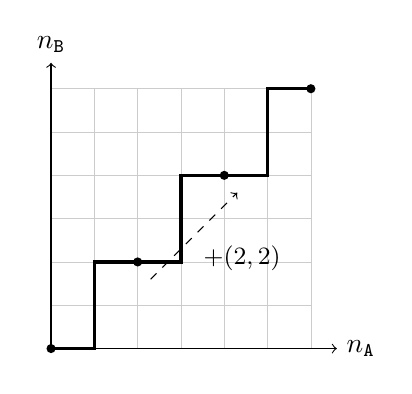
\begin{tikzpicture}[scale=0.55]
\draw[help lines,black!20] (0,0) grid (6,6);
\draw[->] (0,0) -- (6.6,0) node[right] {$n_{\mathtt A}$};
\draw[->] (0,0) -- (0,6.6) node[above] {$n_{\mathtt B}$};
% w_AB = ABBA ABBA ABBA
\draw[very thick] (0,0) -- (1,0) -- (1,2) -- (2,2) -- (3,2) -- (3,4) -- (4,4) -- (5,4) -- (5,6) -- (6,6);
\foreach \p in {(0,0),(2,2),(4,4),(6,6)} \fill \p circle (3pt);
\draw[dashed,->] (2.3,1.6) -- node[below right] {\small $+(2,2)$} (4.3,3.6);
\end{tikzpicture}
\caption{The shadow of the necklace of Figure~\ref{fig:blocks} on the
$\mathtt{A},\mathtt{B}$ plane. The projection is
$w_{\mathtt{AB}}=(\mathtt{ABBA})^3$, so the path repeats after every
shift by $(2,2)$.}\label{fig:shadow}
\end{figure}

\begin{proof}
Each $w_{xy}=v^q$ shows that $q$ divides $n_x$; put $s_x=n_x/q$ and
$B=\sum_x s_x=|w|/q$. Work with $W=ww$, whose two-letter projections are
$2q$-th powers of the same words, and let $f(t)\in\mathbb{Z}^k$ count the
letters among the first $t$ letters of $W$. The points $f(0),f(1),\dots$
form a chain: if $t<t'$ then $f(t)\le f(t')$ in every coordinate. Fix
$t\le|w|$ and put $p=f(t)+s$. We show $f(t+B)=p$.

First, every shadow of $p$ lies on the corresponding shadow path. The
point $(f_x(t),f_y(t))$ is the count of $x$s and $y$s in a prefix of
$W_{xy}$ of length $j\le|w_{xy}|$, and in a $2q$-th power of $v$ the
prefix of length $j+|v|$ contains one more copy's worth of letters, so it
has counts $(p_x,p_y)$. That prefix of $W_{xy}$ comes from a prefix of
$W$, so $(p_x,p_y)=(f_x(t'),f_y(t'))$ for some $t'$.

Now suppose $f(t+B)\ne p$. Both have coordinate sum $t+B$, so some
coordinate $x$ has $f_x(t+B)>p_x$ and another coordinate $y$ has
$f_y(t+B)<p_y$. Take $t'$ with $(f_x(t'),f_y(t'))=(p_x,p_y)$. Since
$f_x(t')<f_x(t+B)$, the chain property forces $t'<t+B$, and then
$f_y(t')\le f_y(t+B)<p_y$, a contradiction.

So $f(t+B)=f(t)+s$ for every $t\le|w|$. Comparing the steps at $t$ and
$t+B$ shows that the letter in position $t+B$ of $w$ equals the letter in
position $t$ whenever both exist. Hence $w$ has period $B$, and as
$|w|=qB$, it is the $q$-th power of its first $B$ letters.
\end{proof}

\section{Constructions}

The upper bounds come from interleaving pairs of colours, each pair with
a rhythm of its own. Figure~\ref{fig:blocks} shows the case $k=4$, using
Weiss's example
\[
\mathtt{ABCD\ BACD\ ABDC\ BACD\ ABCD\ BADC}.
\]
It has six blocks. In each block the pair $\mathtt{A},\mathtt{B}$ appears
as $\mathtt{AB}$ or $\mathtt{BA}$, alternating, so its pattern has period
$2$; the pair $\mathtt{C},\mathtt{D}$ appears as $\mathtt{DC}$ in every
third block and as $\mathtt{CD}$ otherwise, period $3$. Removing $\mathtt{C}$ or
$\mathtt{D}$ destroys the second rhythm and leaves a word of period $2$
blocks, a cube. Removing $\mathtt{A}$ or $\mathtt{B}$ leaves period $3$
blocks, a square. The necklace itself only repeats when both rhythms
line up, after $\operatorname{lcm}(2,3)=6$ blocks, which is the whole
necklace.

\begin{figure}[ht]
\centering
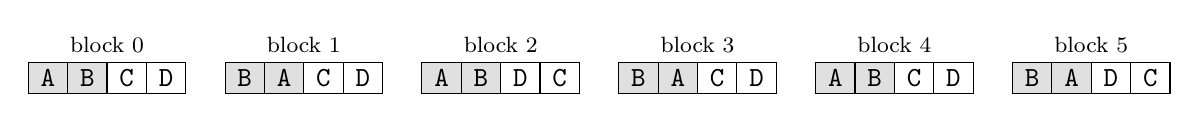
\begin{tikzpicture}[x=5mm,y=5mm]
\foreach \j in {0,...,5}{
  \node[font=\footnotesize] at (\j*5+2,1.25) {block \j};
}
\def\row#1#2{%
  \foreach \c [count=\i from 0] in {#2}{%
    \pgfmathsetmacro\x{#1*5+\i}
    \ifnum\i<2 \fill[black!12] (\x,0) rectangle +(1,0.8);\fi
    \draw (\x,0) rectangle +(1,0.8);
    \node at (\x+0.5,0.4) {$\mathtt{\c}$};}}
\row0{A,B,C,D}\row1{B,A,C,D}\row2{A,B,D,C}\row3{B,A,C,D}\row4{A,B,C,D}\row5{B,A,D,C}
\end{tikzpicture}
\caption{The shortest precarious necklace with four colours, read left to
right and closed into a circle. The shaded pair $\mathtt{A},\mathtt{B}$
swaps every block; the pair $\mathtt{C},\mathtt{D}$ is reversed only in
blocks $2$ and $5$.}\label{fig:blocks}
\end{figure}

In general give the $i$-th pair of colours, $\{x_i,y_i\}$, the prime
$p_i$, and let block $j$ list the pairs in order, pair $i$ as $x_iy_i$ if
$p_i$ divides $j$ and as $y_ix_i$ otherwise. (Weiss's example follows the
mirror rule for the second pair, which works equally well.)

\emph{Odd $s=2h+1$.} Use $h+1$ pairs and $P_{h+1}$ blocks, and put the
remaining $k-2h-2$ colours at the end of every block, in a fixed order.
Each colour appears once per block, so the length is $k\,P_{h+1}$. A set
of $s$ colours cannot contain all $2h+2$ pair colours, so it misses a
colour of some pair $i$. Keeping only that set, what remains of pair $i$
no longer depends on the block, and the blocks repeat with period
$P_{h+1}/p_i$: the kept word is a $p_i$-th power. The whole word is not a
proper power. A rotation fixing it moves every colour by the same number
of blocks, since each colour occurs once per block, and pair $i$ only
returns to its pattern after a multiple of $p_i$ blocks, so the shift is
a multiple of $P_{h+1}$.

\emph{Even $s=2h$.} Use $h$ pairs and $P_h\,p_{h+1}$ blocks, so the
indices $j$ run up to $P_h\,p_{h+1}-1$, and put a cluster of the
remaining $k-s$ colours, in a fixed order, before each group of
$p_{h+1}$ consecutive blocks. There are $P_h$ groups, each of length
$k-s+2h\,p_{h+1}$, so the length is
$P_h(k-s)+2h\,P_{h+1}=s\,P_{h+1}+(k-s)\,P_h$. A set of $s$ colours either
misses a colour of some pair $i$, and then the groups repeat with period
$P_h/p_i$, or it consists of exactly the $2h$ pair colours, and then it
keeps the blocks alone, which repeat with period $P_h$ blocks. For the
whole word, suppose it equals $v^r$ with $r\ge2$. A cluster colour occurs
$P_h$ times, so some prime factor $p$ of $r$ divides $P_h$, say $p=p_i$.
Pair $i$ would then repeat after $P_h\,p_{h+1}/p_i$ blocks, which is
impossible because $p_i$ divides neither $P_h/p_i$ nor $p_{h+1}$.

For $s=k-1$ these are the constructions behind Theorem~\ref{thm:main}:
pairs alone when $k$ is even, and a single extra colour before every
$p_{m+1}$ blocks when $k=2m+1$. Weiss's example for $k=5$ has exactly
this shape, with six groups of five blocks.

\begin{remark}
For $s=k-1$ the constructions satisfy more than is asked: removing any
nonempty set of colours, not just one, leaves a symmetric necklace. So
requiring every deletion to be symmetric does not change $a(k)$.
\end{remark}

\section{The lower bound}

Let $N$ be an $s$-precarious necklace with $k$ colours, $1\le s<k$, and
let $\mathcal K$ be the set of $s$-element sets of colours. For each
$S\in\mathcal K$ the projection $N_S$ is a proper power $v^{r}$; choose a
prime $c(S)$ dividing its exponent. By Lemma~\ref{lem:divide}, $c(S)$
divides $n_x$ for every $x\in S$.

\emph{Avoided pairs.} Fix a prime $q$. If every pair of colours lay in
some $S$ with $c(S)=q$, then by Lemma~\ref{lem:divide} each two-letter
projection would be a projection of a $q$-th power, hence a $q$-th power
itself, and by Lemma~\ref{lem:pairs} $N$ would be a $q$-th power,
contradicting Lemma~\ref{lem:rotation}. So each prime $q$ has an
\emph{avoided pair} $e_q$ of colours that lies in no $S$ with $c(S)=q$.

\emph{Spanning.} For a colour $x$, let $Q_x$ be the set of primes $c(S)$
over the sets $S\ni x$. Then $n_x$ is divisible by every prime in $Q_x$,
so $n_x\ge P_{|Q_x|}$, since distinct primes multiply to at least the
product of the same number of smallest primes. Let $U_x$ be the union of
$\{x\}$ and the avoided pairs $e_q$, $q\in Q_x$. If $|U_x|\le s$, some
$S\in\mathcal K$ contains $U_x$; then $x\in S$, so $c(S)\in Q_x$, and $S$
contains the avoided pair of $c(S)$, which is impossible. Therefore
\begin{equation}\label{eq:span}
s+1\le|U_x|\le 1+2|Q_x|.
\end{equation}

\emph{Odd $s=2h+1$.} By~\eqref{eq:span}, $|Q_x|\ge h+1$ for every colour,
so $|N|=\sum_x n_x\ge k\,P_{h+1}$, which is~\eqref{eq:closed}.

\emph{Even $s=2h$.} Now~\eqref{eq:span} only gives $|Q_x|\ge h$. Call $x$
\emph{heavy} if $|Q_x|\ge h+1$ and \emph{light} otherwise. A colour $y$
that lies in some $S$ whose prime's avoided pair contains $y$ is heavy:
then $y$ already belongs to one of its own avoided pairs, and the first
inequality in~\eqref{eq:span} improves to $s+1\le 2|Q_y|$.

Suppose $x$ is light. Then both inequalities in~\eqref{eq:span} are
equalities: the $h$ avoided pairs of $Q_x$ are disjoint, they miss $x$,
and together with $x$ they form a set $V$ of $s+1$ colours. Take
$y\in V\setminus\{x\}$, lying in the avoided pair $e_q$, and let $z$ be
its partner in that pair. The set $V\setminus\{z\}$ belongs to
$\mathcal K$ and contains $x$, so its prime lies in $Q_x$, and its
prime's avoided pair is not inside it. Every avoided pair of $Q_x$ other
than $e_q$ is inside it, so its prime is $q$. Since $y\in V\setminus\{z\}$ and $y\in e_q$, the colour $y$ is
heavy.

Thus a single light colour forces the $s$ colours of $V\setminus\{x\}$ to
be heavy. If there is a light colour,
$|N|\ge s\,P_{h+1}+(k-s)\,P_h$; if there is none, $|N|\ge
k\,P_{h+1}$, which is larger. This is~\eqref{eq:closed}, and together
with the constructions it proves Theorem~\ref{thm:general}.
Theorem~\ref{thm:main} is the case $s=k-1$: for $k=2m$ the formula reads
$(2m-1)P_m+P_m=2m\,P_m$, and for $k=2m+1$ it reads $2m\,P_{m+1}+P_m$.

\section{Formal verification}

Every statement above has been checked in the Lean~4 proof assistant
\cite{Lean4} with the Mathlib library \cite{Mathlib}, using only Lean's
standard axioms. The formalisation covers Lemmas~\ref{lem:rotation}
to~\ref{lem:pairs}, both constructions for all $k$ and $s$, the lower
bound, Theorems~\ref{thm:main} and~\ref{thm:general}, the identification
of precarious with $(k-1)$-precarious, and the remark. As a check that
the statements say what they should, each of 39 small changes to them
(an off-by-one in a bound, a wrong exponent, a swapped hypothesis) was
confirmed to make the file fail to compile. The Lean files, the
mutation tests and the programs that check the constructions and
Table~\ref{tab:values} independently are at~\cite{repo}.

\section*{Acknowledgements}
The question and the examples for $k\le5$ are Philip Weiss's. The proofs,
the programs, the Lean formalisation and a draft of the text were
developed with Claude Opus~5.5 (Anthropic). A second AI system, used for
an independent check of the general formula, suggested the shorter
argument for the even case of the lower bound in Section~4. The author is
responsible for the content.

\begin{thebibliography}{9}

\bibitem{Lean4} L.~de~Moura and S.~Ullrich, The Lean~4 theorem prover and
programming language, in: A.~Platzer and G.~Sutcliffe (eds.),
\emph{Automated Deduction -- CADE~28}, Lecture Notes in Comput. Sci.
12699, Springer, 2021, pp.~625--635.
\href{https://doi.org/10.1007/978-3-030-79876-5_37}{doi:10.1007/978-3-030-79876-5\_37}.

\bibitem{Mathlib} The mathlib Community, The Lean mathematical library,
in: \emph{Proceedings of the 9th ACM SIGPLAN International Conference on
Certified Programs and Proofs (CPP 2020)}, ACM, 2020, pp.~367--381.
\href{https://doi.org/10.1145/3372885.3373824}{doi:10.1145/3372885.3373824}.

\bibitem{MO} P.~Weiss, How short can a precarious necklace be?,
MathOverflow question 515996, 12 October 2026,
\url{https://mathoverflow.net/q/515996} (accessed 13 October 2026).

\bibitem{repo} V.~Jandhyala, Precarious necklaces: Lean proofs and code,
\url{https://github.com/jvvk/mathematics/tree/main/precarious-necklaces}.

\end{thebibliography}
\end{document}
